\chapter{RESULTADOS}

Este capítulo apresenta os resultados obtidos a partir das simulações e do processamento do sistema de transmissão em banda dupla concorrente. A análise foca no desempenho dos coeficientes do filtro FIR otimizado via método de Powell e na avaliação da envoltória do sinal no domínio do tempo.

\section{Otimização dos Coeficientes do Filtro}

A principal premissa para a viabilidade da implementação em hardware foi a restrição da ordem do filtro. O algoritmo de otimização foi configurado para operar com um comprimento de filtro igual a 9 amostras ($C = 9$). A Figura \ref{fig:coef_otimizados} apresenta a disposição final das amplitudes da resposta ao impulso após a convergência do método de Powell. Observa-se a simetria característica esperada para filtros de fase linear, garantindo que o processamento não insira distorções de fase na informação transmitida.

\begin{figure}[H]
	\centering
	\caption{Resposta ao impulso do filtro FIR otimizado ($C=9$).}
	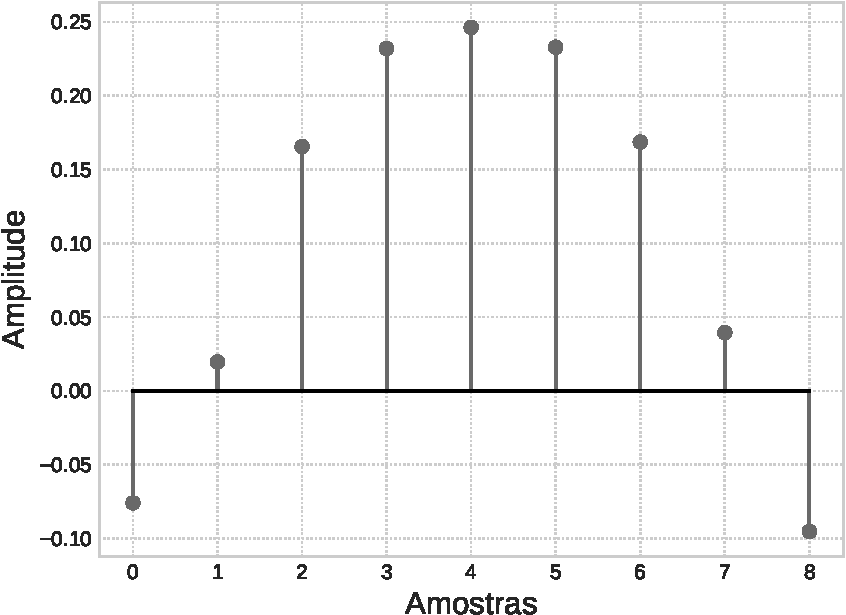
\includegraphics[width=0.8\linewidth]{fig/coeficientes_otimizados.pdf}
	\label{fig:coef_otimizados}
\end{figure}

\section{Análise da Envoltória no Domínio do Tempo}

Para validar a eficácia do filtro otimizado, avaliou-se o erro entre a envoltória do sinal saturado ideal (alvo) e a envoltória do sinal efetivamente filtrado. 

Em uma abordagem inicial sem a otimização refinada dos coeficientes, a filtragem resultava em um desvio perceptível. A Figura \ref{fig:compara_inicial} mostra o comportamento  das envoltórias pré-saturação, saturada e filtrada, acompanhada do gráfico da diferença entre elas. Neste cenário, a diferença média calculada entre a envoltória saturada e a filtrada foi de $4.141 \times 10^{-2}$ V.

\begin{figure}[H]
	\centering
	\caption{Comparação das envoltórias e erro associado (antes da otimização plena).}
	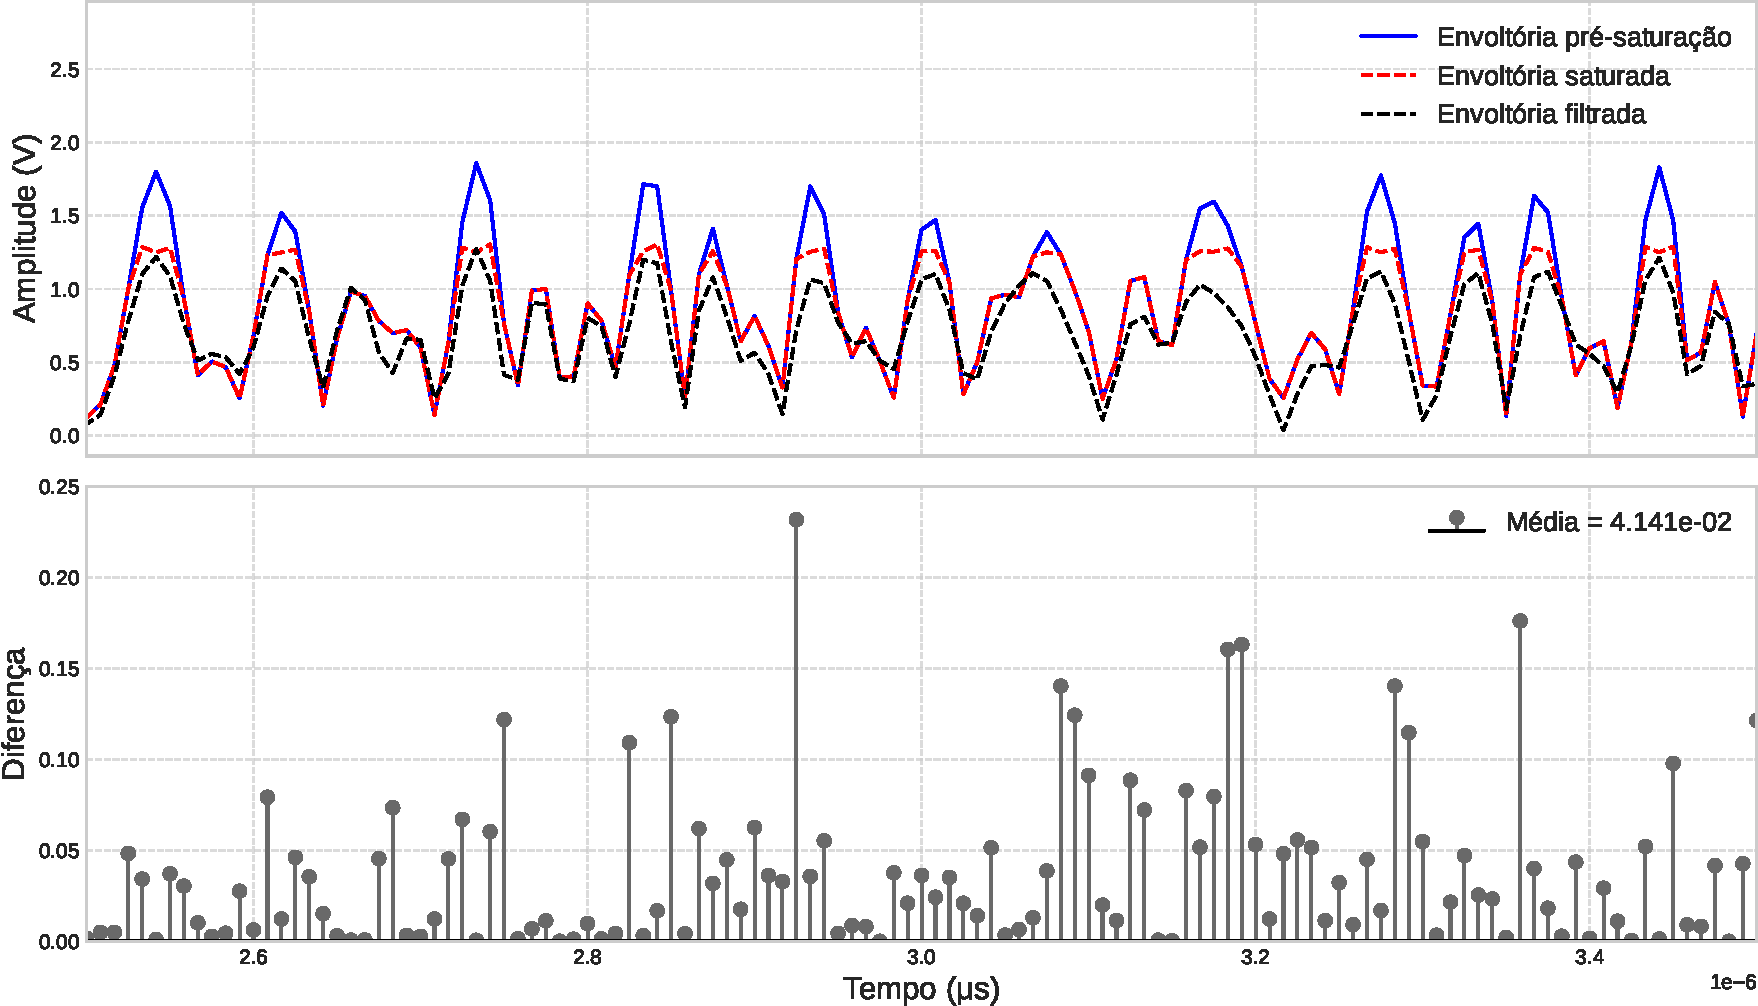
\includegraphics[width=0.75\linewidth]{fig/compara_envoltoria.pdf}
	\label{fig:compara_inicial}
\end{figure}

Após a aplicação do método de Powell utilizando a média das respostas das máscaras, como chute inicial, obteve-se uma melhoria significativa. Conforme indicado na Figura \ref{fig:compara_otimizada}, o sinal filtrado sobrepõe-se com alta fidelidade ao sinal saturado, ou seja, o abjeto de comparação. A eficácia do método de otimização é matematicamente comprovada pela redução na diferença ponto a ponto das envoltórias, que atingiu uma média de $8.649 \times 10^{-5}$ V. Essa queda de ordens de grandeza no erro acaba por validar a capacidade do filtro em limitar a amplitude sem degradar a forma de onda estabelecida no processo de saturação.

\begin{figure}[H]
	\centering
	\caption{Comparação das envoltórias e erro associado utilizando os coeficientes otimizados.}
	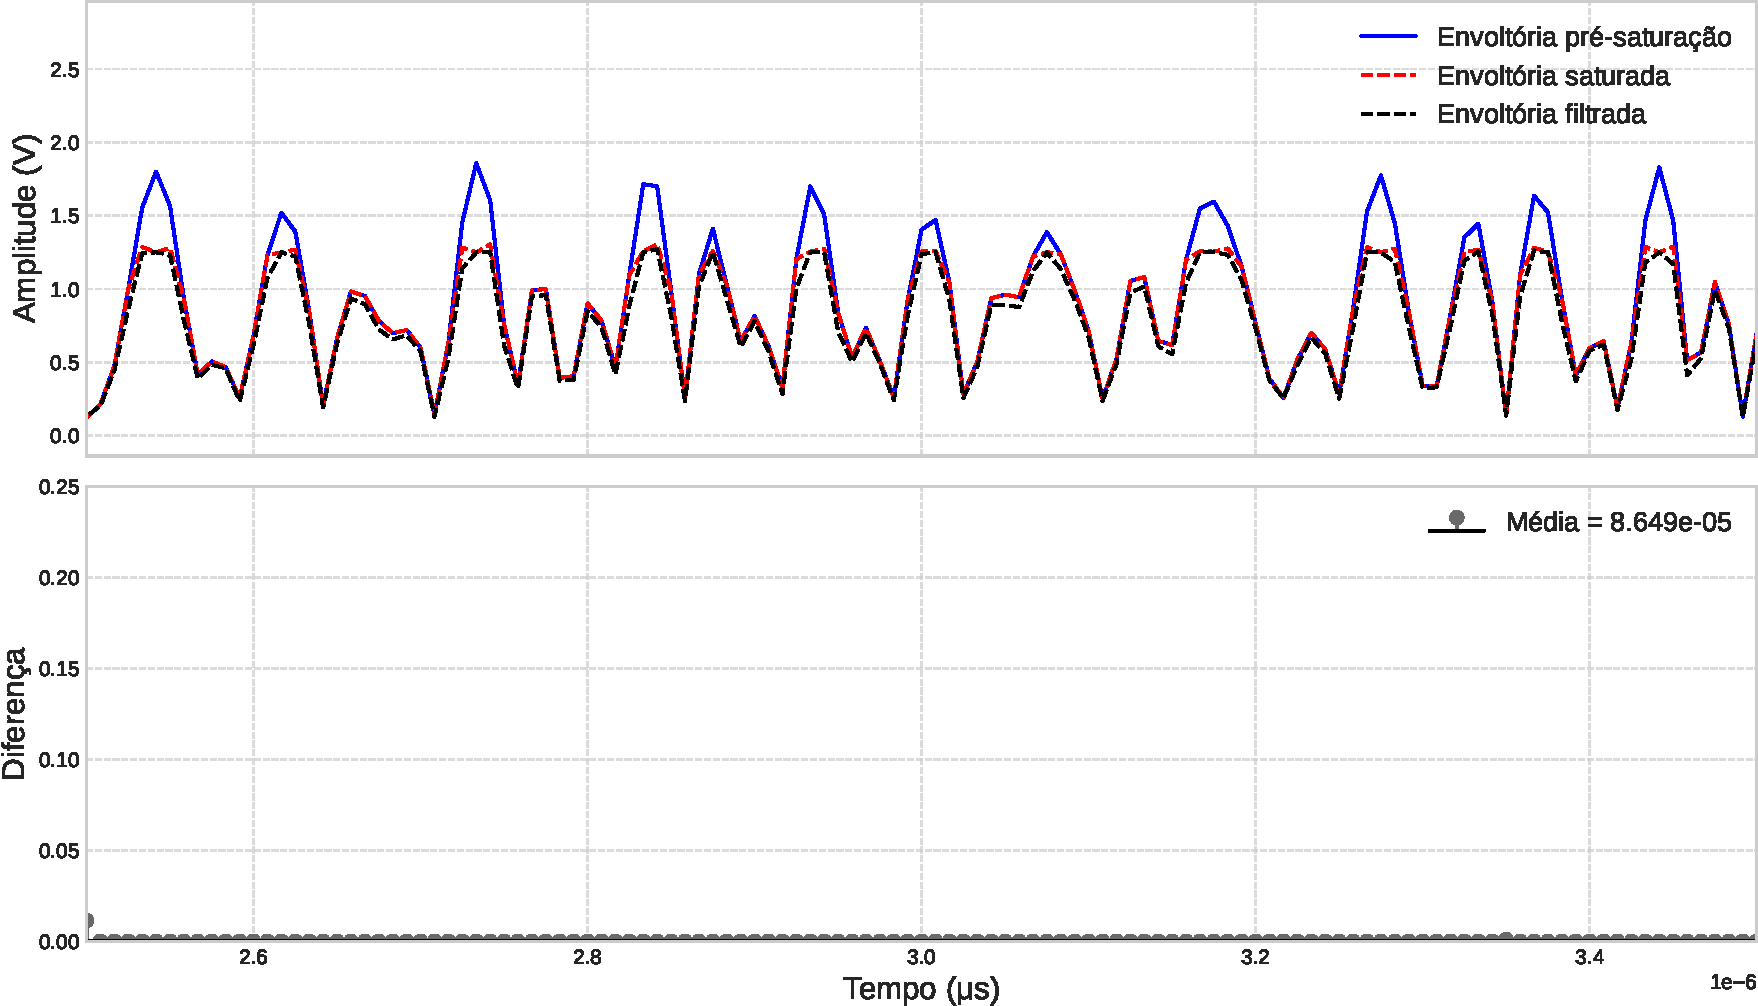
\includegraphics[width=0.75\linewidth]{fig/compara_envoltoria_otimizada.pdf}
	\label{fig:compara_otimizada}
\end{figure}

O comportamento das envoltórias é mais bem explorado pela Figura \ref{fig:envoltoria_mascara}, que demonstra a consistência do nível de tensão mantido pelo sinal filtrado ao longo do tempo.

\begin{figure}[H]
	\centering
	\caption{Detalhamento do comportamento temporal das envoltórias pré-saturação, saturada e filtrada.}
	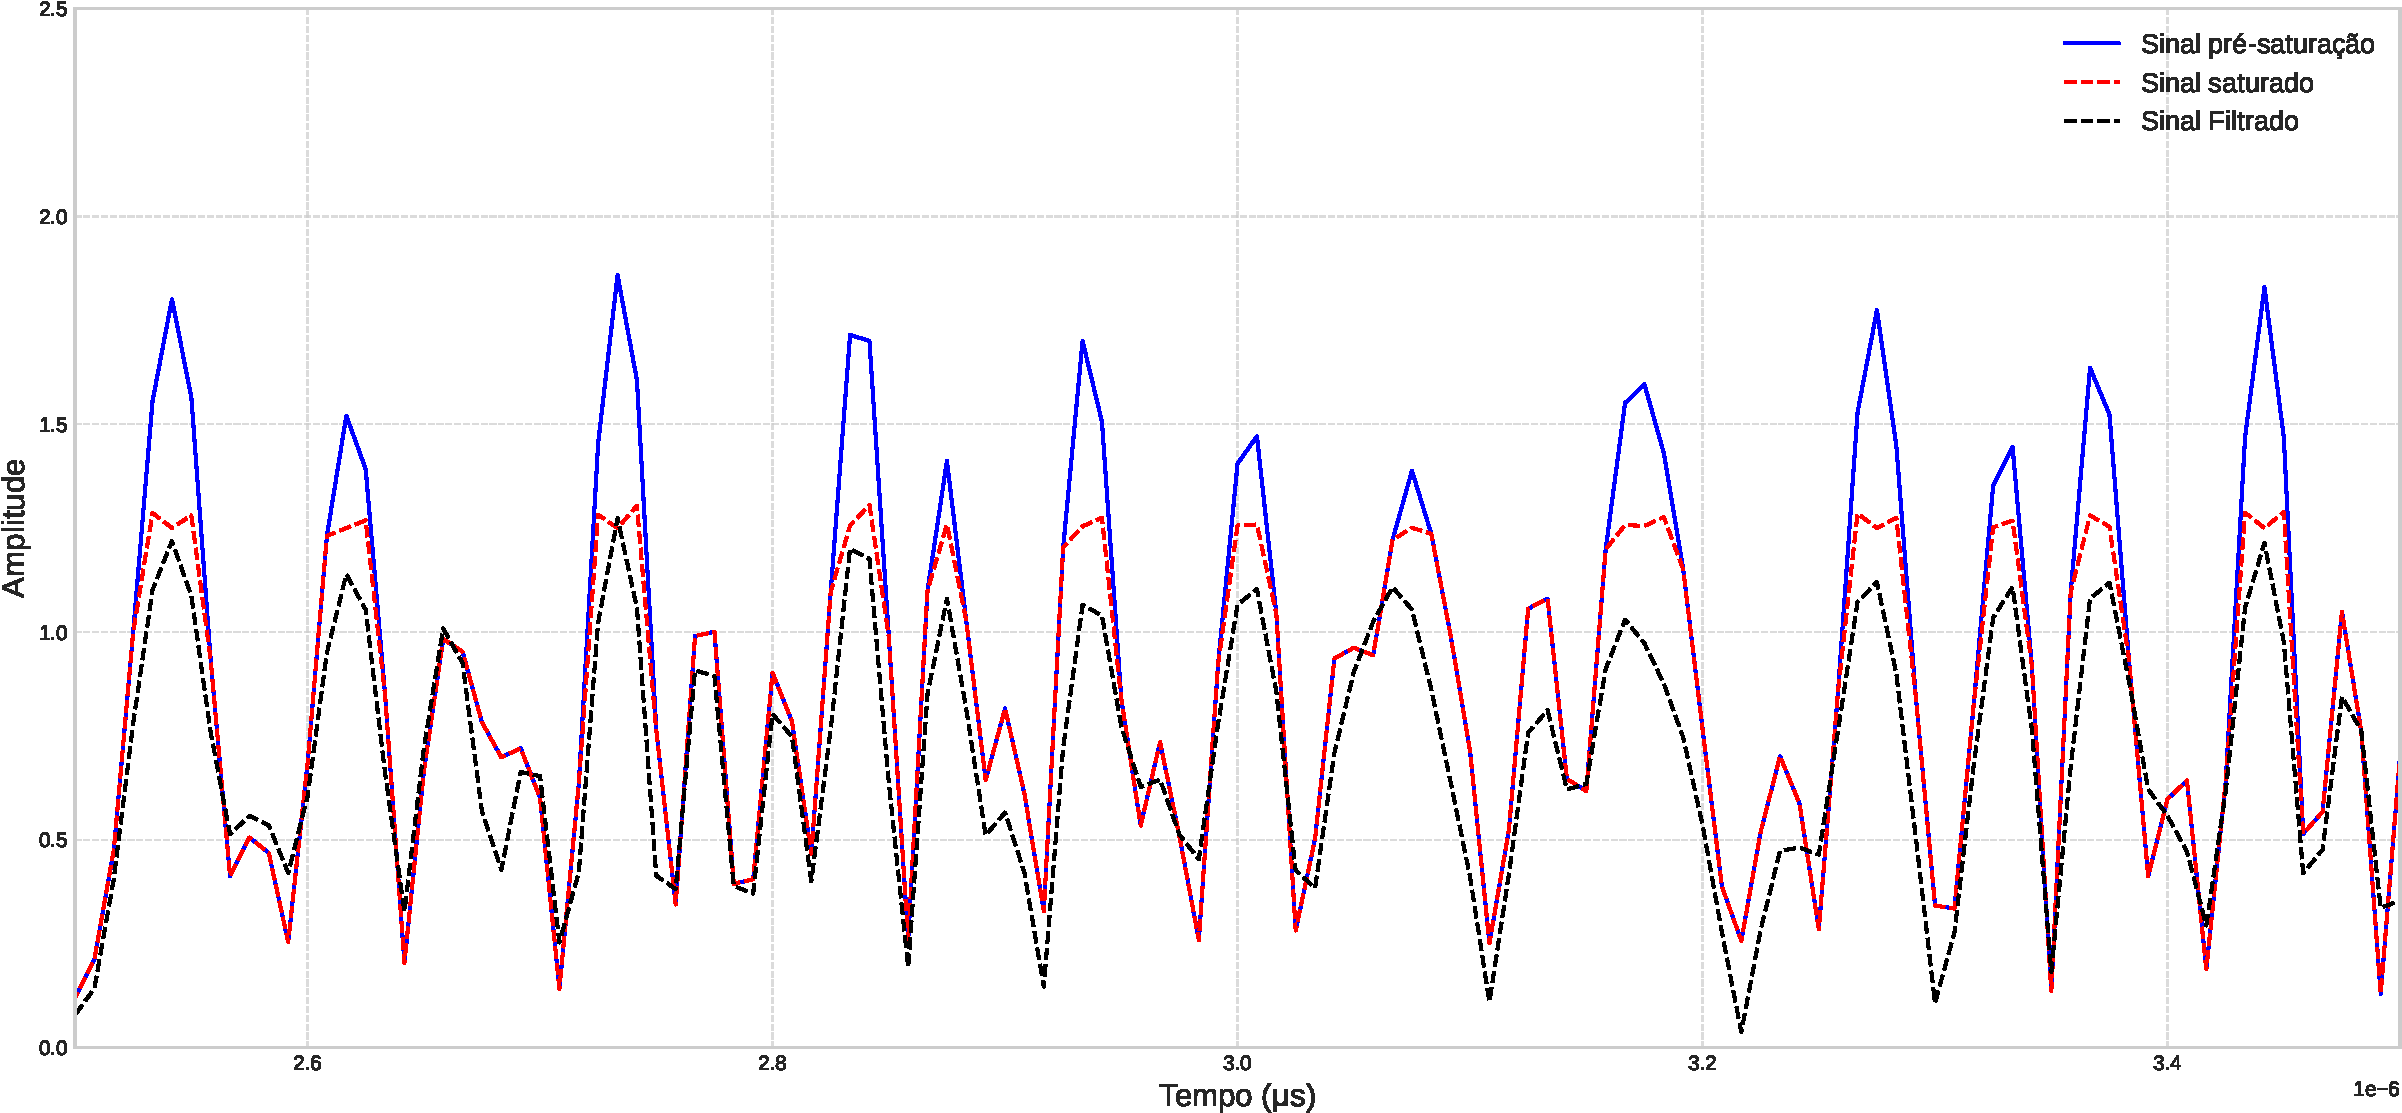
\includegraphics[width=0.9\linewidth]{fig/envoltoria_comparação_mascara.pdf}
	\label{fig:envoltoria_mascara}
\end{figure}

Quando analisado a curva de PSD, Densidade Espectral de Potência, é possível observar por meio da Figura \ref{fig:psd_otimizado} que o espectro de frequência do sinal filtrado é limitado dentro dos limites desenhados pela norma. A frequência do sinal é atenuado conforme se afasta da frequência central, no caso em banda base de zero hertz. 

\begin{figure}[H]
	\centering
	\caption{Comportamento da Densidade Espectral de Potência da envoltória equivalente}
	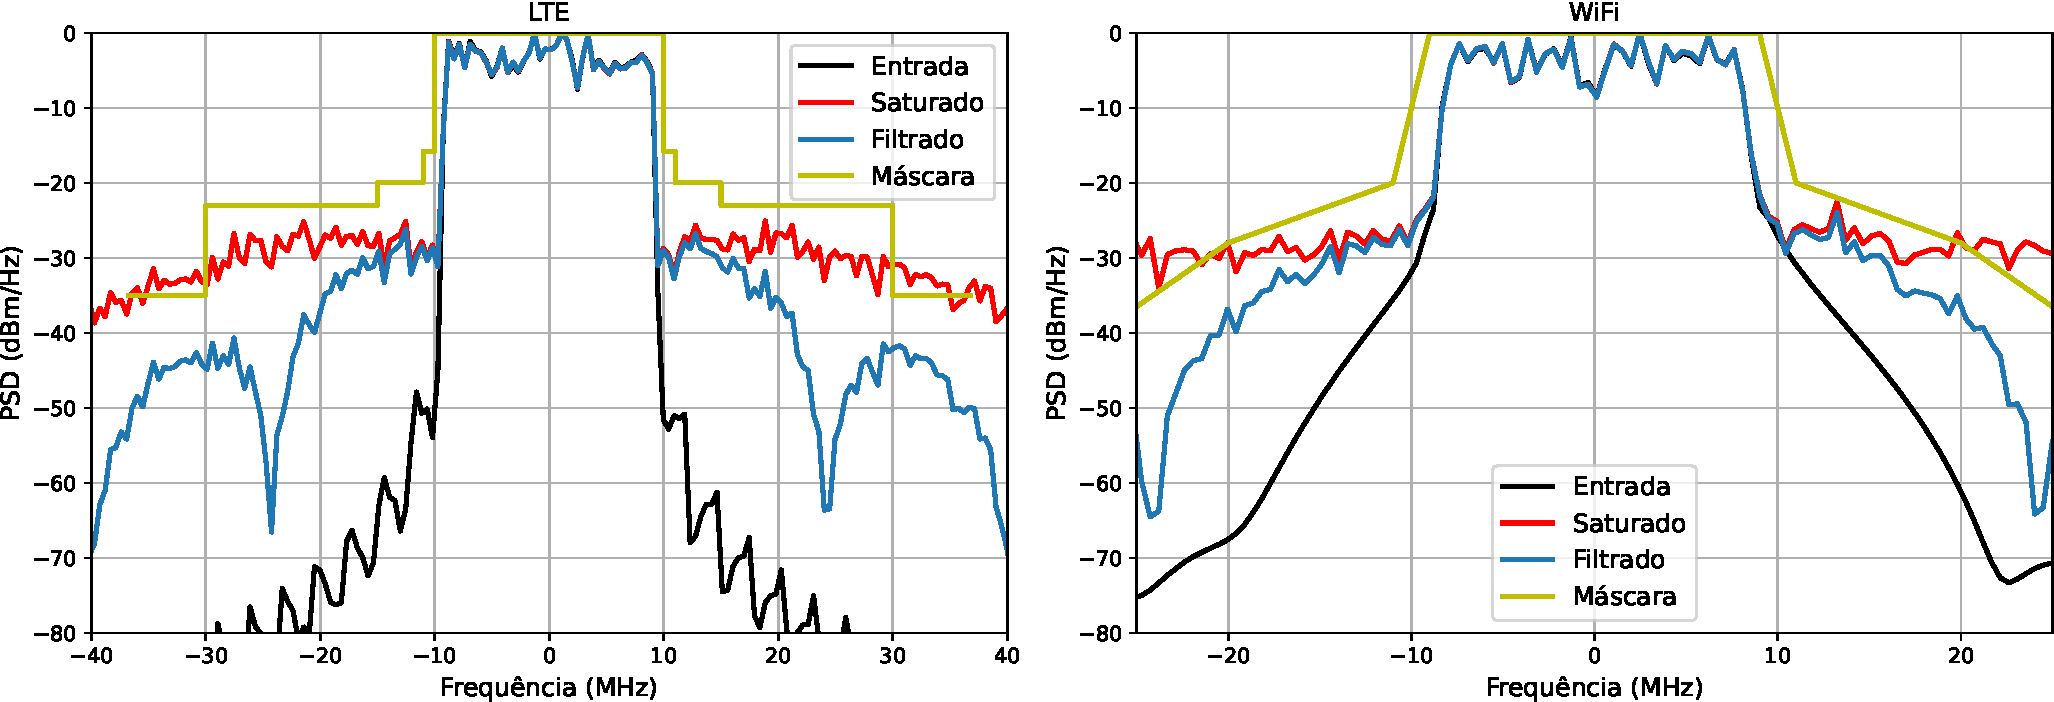
\includegraphics[width=0.9\linewidth]{fig/psd_otimizado.pdf}
	\label{fig:psd_otimizado}
\end{figure}



\section{Desempenho dos Sinais Individuais (Banda Dupla)}

Dado que o sistema processa um sinal composto por duas portadoras distintas, é imprescindível garantir que a recuperação e o tratamento do sinal excedente preservem a integridade de cada banda individualmente. 

A Figura \ref{fig:sinais_separados} detalha o comportamento no domínio do tempo para as bandas Wi-Fi e LTE de forma isolada. É possível observar que, para ambos os padrões, as formas de onda filtradas acompanham as trajetórias dos sinais saturados tidos como base. A técnica de repartição proporcional de soma, aliada ao filtro otimizado, demonstrou ser bem-sucedida em impedir distorções, assegurando que as componentes de alta frequência e os picos de cada canal fossem ceifados de maneira controlada.

\begin{figure}[H]
	\centering
	\caption{Formas de onda individuais para os canais Wi-Fi e LTE após a separação e filtragem otimizada.}
	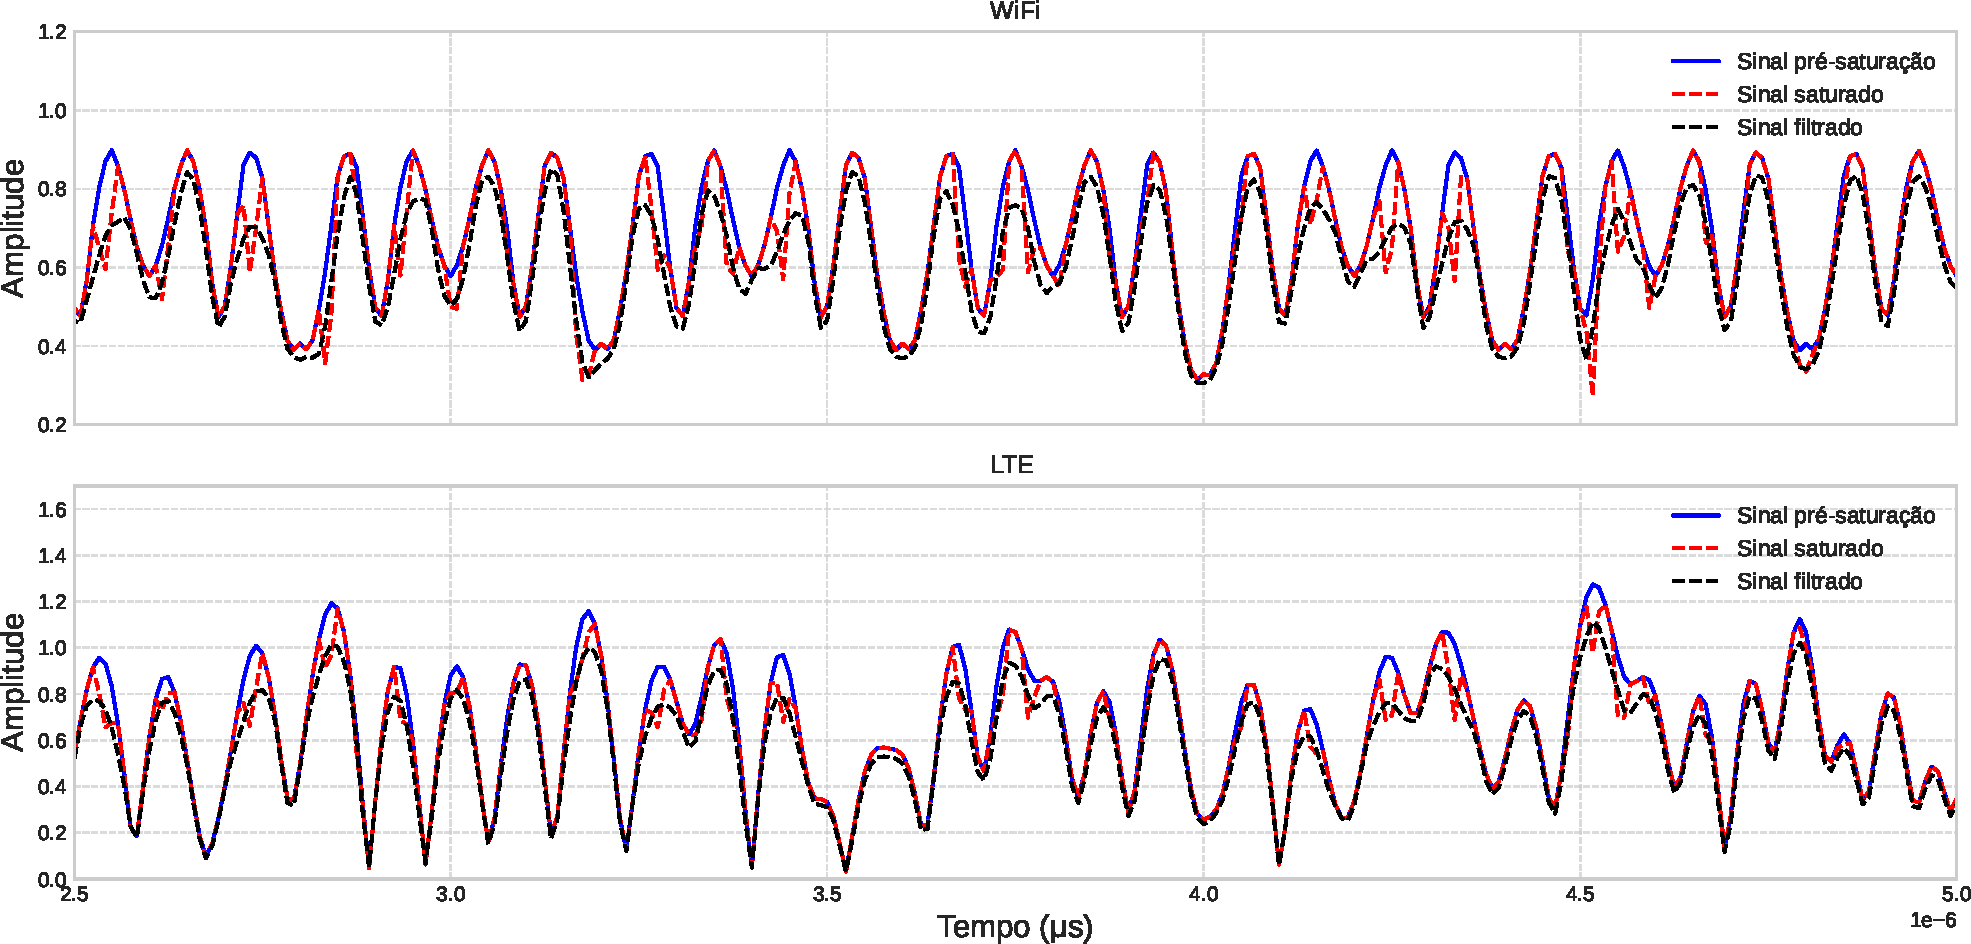
\includegraphics[width=0.9\linewidth]{fig/compara_envoltoria_sinais_otimizado_separados.pdf}
	\label{fig:sinais_separados}
\end{figure}

As Tabelas \ref{tab1} e \ref{tab2} resume, respectivamente, os indicadores de EVM  e PAPR avaliados nas etapas de saturação e filtragem. A análise dessas métricas demonstra que a arquitetura proposta proporcionou um tratamento adequado ao sinal, sem acarretar degradação na qualidade da modulação. No que tange ao EVM, o Canal 1 (Wi-Fi) exibiu uma ligeira melhoria, apresentando uma redução de 0,13 pontos percentuais após a filtragem, enquanto o Canal 2 (LTE) permaneceu inalterado quando comparado ao sinal apenas saturado.

\renewcommand{\arraystretch}{1.3} 
\begin{table}[ht!]
	\centering
	\small
	\caption{Resultados do EVM para os sinais saturados e filtrados dos canais 1 e 2.}
	\begin{tabular}{cccc}
		\toprule
		& \textbf{Com filtro} & \textbf{Sem filtro} \\
		\midrule
		\textbf{Canal 1} & 7,13\% & 7,26\% \\
		\textbf{Canal 2} & 8,02\% & 8,02\% \\
		\bottomrule
	\end{tabular}
	\label{tab1}
\end{table}

Em relação à PAPR, a avaliação individual de cada canal revelou variações marginais, o que atesta a preservação da integridade das informações em ambas as bandas. Por outro lado, ao observar a envoltória complexa equivalente, constata-se que a filtragem introduziu um acréscimo de 1,03 dB na PAPR em comparação ao sinal estritamente saturado. Esse comportamento indica que, embora o filtro restitua uma pequena fração dos picos originais para conter o espalhamento espectral, o sistema como um todo ainda mantém um valor de amplitude média elevada.

\begin{table}[H]
	\centering
	\small
	\caption{PAPR dos sinais não-saturado, saturado e filtrado dos canais 1, 2 e envoltória equivalente.}
	\begin{tabular}{c|ccc} \toprule
		& \textbf{\begin{tabular}[c]{@{}c@{}}PAPR\\ Canal 1\end{tabular}} & \textbf{\begin{tabular}[c]{@{}c@{}}PAPR\\ Canal 2\end{tabular}} & \textbf{\begin{tabular}[c]{@{}c@{}}PAPR\\ Envoltória Eq.\end{tabular}} \\ \midrule
		\textbf{Não-saturado} & 8,43 dB & 8,24 dB & 9,09 dB \\
		\textbf{Saturado} & 8,89 dB & 8,03 dB & 5,28 dB \\
		\textbf{Filtrado} & 8,09 dB & 7,29 dB & 6,31 dB \\  \bottomrule
	\end{tabular}
	\label{tab2}
\end{table}
